\documentclass[12pt,a4paper]{ctexart}

\usepackage[UTF8]{ctex}
\usepackage{geometry}
\usepackage{graphicx}
\usepackage{xcolor}
\usepackage{tikz}
\usepackage{fontspec}
\usepackage{setspace}
\usepackage{enumitem}
\usepackage{booktabs}
\usepackage{array}
\usepackage{longtable}
\usepackage{hyperref}
\usepackage{fancyhdr}
\usepackage{titlesec}
\usepackage{multicol}
\usepackage{xurl}
\usepackage{tocloft}

\renewcommand{\cfttoctitlefont}{\hfill\bfseries\Large}
\renewcommand{\cftaftertoctitle}{\hfill}
\geometry{left=2.5cm,right=2.5cm,top=2.5cm,bottom=2.5cm}

\definecolor{black}{RGB}{0,0,0}
\definecolor{mainblue}{RGB}{0,82,147}
\definecolor{accentgold}{RGB}{180,140,60}
\definecolor{lightgray}{RGB}{245,245,245}
\definecolor{darkgray}{RGB}{80,80,80}
\definecolor{mainred}{RGB}{230,1,45}

\hypersetup{
    colorlinks=true,
    linkcolor=black,
    urlcolor=mainblue,
    citecolor=mainblue,
    pdfborder={0 0 0}
}

\pagestyle{fancy}
\fancyhf{}
\fancyhead[L]{\small\color{darkgray}\textbf{量子行业每周新闻洞察}}
\fancyhead[R]{\small\color{darkgray}\textbf{总第181期}}
\fancyfoot[C]{\thepage}
\renewcommand{\headrulewidth}{0.4pt}
\renewcommand{\footrulewidth}{0pt}

\titleformat{\section}
    {\Large\bfseries\color{mainred}}
    {\thesection、}{0em}{}
\titleformat{\subsection}
    {\large\bfseries\color{mainred}}
    {\thesubsection、}{0em}{}

\newcolumntype{L}[1]{>{\raggedright\arraybackslash}p{#1}}
\newcolumntype{C}[1]{>{\centering\arraybackslash}p{#1}}

\begin{document}

% ==================== 封面 ====================
\begin{titlepage}
\begin{tikzpicture}[remember picture,overlay]
    \fill[mainred] ([yshift=-0.5cm]current page.north west) rectangle ([yshift=-1.2cm]current page.north east);
    \fill[mainred] ([yshift=1.2cm]current page.south west) rectangle ([yshift=0.5cm]current page.south east);
\end{tikzpicture}

\vspace*{4cm}

\begin{center}
    {\fontsize{44}{52}\selectfont\bfseries\color{black} \textbf{量子行业每周新闻洞察}}

    \vspace{0.8cm}
    
    {\fontsize{16}{22}\selectfont\color{darkgray} 2026.05.23 — 2026.05.29 }
    {\fontsize{16}{22}\selectfont\color{darkgray} \textbf{WEEKLY NEWS}}
    
    \vspace{1.5cm}
    
    {\fontsize{20}{26}\selectfont\color{mainred}\textbf{（总第\textbf{ 181 }期）}}
    
    \vspace{4cm}
    
    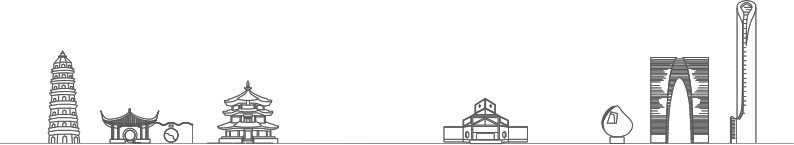
\includegraphics[width=\textwidth]{Cover_Suzhou.png}
    
    \vfill
    
    {\fontsize{12}{16}\selectfont\color{darkgray} 量子科技长三角产业创新中心\\编制：战略情报与成果专利室、产业发展部（理事会办公室）}
\end{center}
\end{titlepage}

% ==================== 目录 ====================
\pagenumbering{roman}
\newpage
\tableofcontents

\newpage

% ==================== 摘要 ====================
\pagenumbering{arabic}
\setcounter{page}{1}
\begin{center}
{\Large\bfseries\color{mainred} 摘\hspace{2em}要}
\end{center}
\addcontentsline{toc}{section}{摘要}


\textbf{ 宏观态势：}

全球量子科技发展正从战略规划转向规模化实施与基础设施构建。欧洲积极构建全大陆量子密钥分发网络，着力打造“量子盾牌”；德国、法国及新加坡等国通过更新路线图、追加巨额投资与出台企业扶助举措，系统性推进产业化和应对量子威胁。同时，量子安全在金融和通信领域的应用加速落地，多国央行与网络安全公司纷纷布局抗量子密码，后量子安全技术已延伸至移动操作系统和加密货币社区。


\textbf{ 科技前沿：}

研究热点聚焦于解决量子计算与量子器件的核心工程难题，并在新材料调控上取得关键突破。科学家们成功将中性原子与集成光子学结合、实现对超导磁涡旋及单分子的量子操控，这些进展为开发更低噪声的量子芯片和新型传感器奠定基础。此外，生成式AI被引入量子线路合成，量子机器学习应用持续拓展，而金刚石超导机制等新发现则为多功能量子器件研发开辟了可能路径，显示出理论探索与实用化工具开发深度协同的趋势。


\textbf{ 产品动态：}

产业界正大力推进量子计算商用化进程和核心组件迭代。中性原子与光量子计算机企业动作频频，通过提升处理器性能、集成控制单元及借壳上市等方式加速市场布局。同时，量子安全生态建设明显提速，涵盖开源芯片分发方案、量子安全密钥管理平台及移动网络加密技术的推出，后量子密码学正加速融入AI机器人和光网络防护。关键设备方面，低温放大器获得首个商业合同，专用制造与测试设备采购活跃，表明量子计算的供应链与工程化支撑体系正在成型。


\textbf{ 企业资讯：}

传统IT巨头与量子软件公司的跨界协作进一步深化，AI在量子计算开发中的实用价值日益显现。甲骨文与Classiq的合作验证了利用人工智能自动生成量子代码并进行大规模仿真的可行性，这一标志性进展预示着量子软件的开发范式正从手工编写向智能化生成转变，有望显著降低企业部署量子应用的门槛，并加速面向具体商业问题的混合算法研发与落地。


\textbf{ 资本运作：}

量子科技领域正迎来一波上市与融资热潮，资本向头部企业和技术聚焦的趋势极为显著。Quantinuum、Terra Quantum等公司纷纷通过传统IPO或SPAC方式谋求上市，估值与募资规模可观。同时，从芬兰算法初创到中国超导量子整机公司，均获得大额融资支持，显示了资本对底层技术突破和整机商业化的双重信心。此外，美国政府通过商务部对PsiQuantum、D-Wave等关键企业注入数亿美元资金，强力驱动本土量子计算核心技术本土化与制造能力升级。




\textbf{ 专利动态：}

本周专利动态涵盖低温环境系统、超导量子测控技术、量子软件与算法、量子科技长三角产业创新中心共4个板块、17条专利。




% ==================== 会议列表 ====================
{
    \newpage
    \section*{ 6月量子科技行业国内、国际会议}
    \addcontentsline{toc}{section}{ 6月量子科技行业国内、国际会议}
    \scriptsize
    \begin{longtable}{C{0.8cm}L{2.5cm}L{3cm}L{7cm}}
        \toprule[1.5pt]
        \textbf{序号} & \textbf{日期} & \textbf{地点} & \textbf{会议名称} \\
        \midrule
        \endfirsthead
        \toprule
        \textbf{序号} & \textbf{日期} & \textbf{地点} & \textbf{会议名称} \\
        \midrule
        \endhead
        \bottomrule
        \endfoot
        
        1 & 6月1日-3日 & 拉勒米, 美国 & 第四届怀俄明大学量子暑期学校 \\
        \midrule[0.05pt]
        
        2 & 6月1日-5日 & 罗利, 美国 & 2026量子机器学习暑期研讨会 \\
        \midrule[0.05pt]
        
        3 & 6月1日-5日 & 普罗维登斯, 美国 & 第57届APS原子、分子与光物理年会 \\
        \midrule[0.05pt]
        
        4 & 6月2日-4日 & 特隆赫姆, 挪威 & 量子自旋电子学 \\
        \midrule[0.05pt]
        
        5 & 6月3日-4日 & 罗切斯特, 美国 & 量子热力学与退相干 \\
        \midrule[0.05pt]
        
        6 & 6月4日-5日 & 东京, 日本 & Q2B：量子价值路线图 \\
        \midrule[0.05pt]
        
        7 & 6月5日 & 格拉斯哥, 英国 & 量子与社会研究研讨沙盒 \\
        \midrule[0.05pt]
        
        8 & 6月7日-12日 & 圣巴巴拉, 美国 & 第八届国际量子纠错会议 \\
        \midrule[0.05pt]
        
        9 & 6月7日-13日 & 克里特岛, 希腊 & 青年原子光学会议 \\
        \midrule[0.05pt]
        
        10 & 6月8日-11日 & 滑铁卢, 加拿大 & 量子光子学 \\
        \midrule[0.05pt]
        
        11 & 6月8日-20日 & 卡尔热斯, 法国 & 量子技术计算与通信暑期学校 \\
        \midrule[0.05pt]
        
        12 & 6月8日-8月14日 & 洛斯阿拉莫斯, 美国 & 2026洛斯阿拉莫斯量子计算暑期学校 \\
        \midrule[0.05pt]
        
        13 & 6月9日 & 巴黎, 法国 & Q-Day量子风险峰会：后量子密码学与量子密钥分发 \\
        \midrule[0.05pt]
        
        14 & 6月10日-12日 & 华沙, 波兰 & Perspektywy科技女性峰会 \\
        \midrule[0.05pt]
        
        15 & 6月10日-12日 & 多恩比恩, 奥地利 & 第四届砷化镓量子点国际研讨会 \\
        \midrule[0.05pt]
        
        16 & 6月10日-12日 & 埃朗根, 德国 & 神经形态计算前沿 \\
        \midrule[0.05pt]
        
        17 & 6月11日 & 杰克逊维尔, 美国 & 量子当下，医疗未来 \\
        \midrule[0.05pt]
        
        18 & 6月15日-17日 & 苏黎世, 瑞士 & 欧洲集成光学会议（ECIO） \\
        \midrule[0.05pt]
        
        19 & 6月15日-18日 & 格拉斯哥, 英国 & Optica Quantum 2.0会议 \\
        \midrule[0.05pt]
        
        20 & 6月15日-18日 & 赫尔辛基, 芬兰 & 仲夏开放量子系统、退相干及量子-经典交叉会议 \\
        \midrule[0.05pt]
        
        21 & 6月15日-18日 & 洛杉矶, 美国 & 量子器件设计研讨会 \\
        \midrule[0.05pt]
        
        22 & 6月16日 & 巴黎, 法国 & 第5届France Quantum \\
        \midrule[0.05pt]
        
        23 & 6月16日-17日 & 伦敦, 英国 & 第5届年度量子商业化全球大会2026 \\
        \midrule[0.05pt]
        
        24 & 6月16日-17日 & 格拉斯哥, 英国 & Optica 2026量子产业峰会——第5届 \\
        \midrule[0.05pt]
        
        25 & 6月21日-25日 & 塞费尔德, 奥地利 & 第57届欧洲原子系统组年度会议（EGAS 57） \\
        \midrule[0.05pt]
        
        26 & 6月21日-26日 & 塞费尔德, 奥地利 & 第7届塞费尔德量子信息研讨会 \\
        \midrule[0.05pt]
        
        27 & 6月21日-7月4日 & 贝纳斯克, 西班牙 & 量子科学：实现 \\
        \midrule[0.05pt]
        
        28 & 6月22日-24日 & 奥斯陆, 挪威 & IQT北欧：变化世界中的量子技术 \\
        \midrule[0.05pt]
        
        29 & 6月26日 & 汉堡, 德国 & 第7届ISC HPC国际研讨会——监控、可观测性与运营数据分析 \\
        \midrule[0.05pt]
        
        30 & 6月26日 & 汉堡, 德国 & 第2届统一计算中心量子资源研讨会（QRUCH） \\
        \midrule[0.05pt]
        
        31 & 6月26日 & 汉堡, 德国 & 第5届量子及混合量子/经典计算方法研讨会 \\
        \midrule[0.05pt]
        
        32 & 6月26日 & 汉堡, 德国 & 科学与工业数字孪生研讨会——从数据科学家到数据中心 \\
        \midrule[0.05pt]
        
        33 & 6月22日-7月3日 & 雷苏什, 法国 & 2026光子与原子暑期学校：量子气体、光-物质相互作用、量子技术 \\
        \midrule[0.05pt]
        
        34 & 6月23日-24日 & 罗马(纽约州), 美国 & 量子国际年度研讨会（Q4I） \\
        \midrule[0.05pt]
        
        35 & 6月23日-26日 & 阿尔加维, 葡萄牙 & 第3届量子安全网络与系统研讨会（QSNS 2026） \\
        \midrule[0.05pt]
        
        36 & 6月25日-26日 & 波士顿, 美国 & Quantum.Tech World \\
        \midrule[0.05pt]
        
        37 & 6月29日-7月1日 & 汉堡, 德国 & 国际计算科学大会量子计算专题 \\
        \midrule[0.05pt]
        
        38 & 6月29日-7月3日 & 贝桑松, 法国 & 第14届欧洲频率与时间研讨会（EFTS） \\
        \midrule[0.05pt]
        
        39 & 6月29日-7月10日 & 阿斯巴雷拉斯, 西班牙 & La Ricotta暑期学校：干草堆中的量子 \\
        \midrule[0.05pt]
        
        40 & 6月30日-7月1日 & 柏林, 德国 & GITEX欧洲 \\
        \midrule[0.05pt]
        
    \end{longtable}
}




% ==================== 宏观态势 ====================
\newpage
\section{宏观态势}
\vspace{-0.5em}
\noindent\rule{\linewidth}{1.5pt}

\subsection{ 美特朗普政府出资20亿入股9家量子企业}

5月21日，美国商务部表示，特朗普政府将向9家量子计算企业合计发放20亿美元扶持资金，相关交易包含美国政府获取股权的条款。根据安排，美国政府将从这笔资金中拨出10亿美元给予IBM。此外，芯片制造商GlobalFoundries将获得3.75亿美元资助，其余多数企业预计获得1亿美元资金，初创公司Diraq的资助金额为3800万美元。一批采用不同技术路径的量子公司也将获得拨款，包括上市公司D-WaveQuantum、RigettiComputing以及Infleqtion等。受此消息刺激，相关上市公司股价在周四盘前交易中大幅上涨，其中IBM和GlobalFoundries均上涨约7\%，RigettiComputing涨超15\%，D-WaveQuantum涨超17\%，IONQ涨超8\%。

\noindent\textbf{报道链接：}\url{https://www.nist.gov/news-events/news/2026/05/department-commerce-announces-letters-intent-9-companies-2-billion}

\subsection{ 德国政府发布新版量子路线图：从研发转向产业规模化 }

2026年05月29日消息，德国联邦教育与研究部（BMFTR）近日正式发布了新版《量子技术路线图》，标志着德国量子政策正从研发向产业规模化发展向的关键转变。该国家量子路线图的核心支柱包括：在工业用例中实现可验证的量子优势以推动商业应用，构建关键子组件的弹性欧洲供应链确保可完全自主，培养具备市场技能的工程师队伍，以及利用“高科技空间”消除生态系统碎片化实现敏捷执行。这一框架将为德国量子技术的产业化落地提供系统性指导。

\noindent\textbf{报道链接：}\url{https://qbn.world/german-government-unveils-quantum-technologies-roadmap-for-its-hightech-agenda/ }

\subsection{ 罗马尼亚将投资超1亿欧元部署该国首台量子计算机 }

2026年05月27日消息，罗马尼亚计划于今年秋季在雅西部署该国首台量子计算机，总投资超过1亿欧元，并将向高校、研究机构及企业开放接入量子计算基础设施的能力。据悉，该项目旨在强化罗马尼亚的量子研究生态，其中罗马尼亚的亚历山德鲁·伊万·库扎大学将在量子技术相关的培训与研究项目中承担核心作用。研究人员表示，该量子计算系统可在网络安全、人工智能、物流、制药及先进材料等领域提供支持，通过执行复杂计算，解决传统计算机难以处理的问题。

\noindent\textbf{报道链接：}\url{https://thequantuminsider.com/2026/05/26/romania-plans-e100-million-quantum-computer-project-in-iasi/ }

\subsection{ 新加坡出台一系列新举措，助力企业应对AI革命与量子威胁双重挑战 }

2026年05月26日消息，新加坡近日宣布了多项新举措，旨在推动企业采用人工智能技术、提升网络韧性，并提前应对量子相关安全风险对电信基础设施带来的挑战。在ATxEnterprise 2026大会上，新加坡数字发展与信息部高级政务部长陈杰豪（音译）公布了“数字企业蓝图”下的新计划，该计划涉及与政府机构、科技公司及电信运营商的合作。这些措施旨在帮助新加坡企业借助AI提高竞争力，同时加强防御网络攻击的能力，并开始为后量子密码时代做准备，确保电信网络在量子计算威胁下仍能保存安全。

\noindent\textbf{报道链接：}\url{https://www.telecompaper.com/news/singapore-expands-quantum-safe-telecom-infrastructure-plans-enterprise-ai-initiatives--1571874 }

\subsection{ 法国重金押注未来：马克龙宣布追加10亿欧元发展量子技术 }

2026年05月26日消息，法国总统马克龙于日前宣布，将追加15.5亿欧元（约17.9亿美元）投资量子计算与半导体领域，并指出欧洲各国应携手推进这两大关键战略技术，以在全球竞争中保持领先地位。在参观巴黎近郊的原子能暨替代能源委员会（CEA）超算中心时，马克龙透露，新资助方案将从“法国2030”计划中拨出10亿欧元用于量子技术，另增加5.5亿欧元支持半导体领域。这笔资金将助力量子计算领域的发展，并补充了法国于2021年投入18亿欧元以加强国家量子战略的承诺。

\noindent\textbf{报道链接：}\url{https://www.france24.com/en/live-news/20260522-france-announces-billion-euro-boost-for-quantum-computing }

\subsection{ 美国伊利诺伊州发布该州首份量子教育全景报告 }

2026年05月25日消息，近日，美国伊利诺伊科技联盟、伊利诺伊经济发展公司、伊利诺伊量子与微电子园区以及芝加哥量子交易所发布了首份联合报告，系统追踪了伊利诺伊州量子人才培养体系的发展情况，进一步体现了该州在全美量子人才发展领域的领先地位。这份名为《伊利诺伊量子人才培养路径图谱：定义量子相关学位与证书的框架》的报告显示，2024年该州共颁发了超过33000个量子相关的学位与证书，较2018年《国家量子倡议法案》通过以来增长33\%，较过去十年累计增长60\%。该报告还指出，伊利诺伊州约占全美量子相关课程完成总量的近5\%。

\noindent\textbf{报道链接：}\url{https://iqmp.org/news/first-of-its-kind-report-positions-illinois-as-national-leader-in-quantum-workforce-development/ }

\subsection{ 巴西推进Quandanga量子通信网络项目，将建首个永久性实验基础设施 }

2026年05月29日消息，巴西国家电信局（Anatel）与军事工程学院（IME）近日举行了一次会晤，以讨论推进Quandanga量子通信网络项目的开发。该项目旨在打造巴西首个永久性实验基础设施，用于研究、测试和演示基于量子及后量子密码技术的安全通信方案。这一合作标志着巴西在量子通信领域迈出关键一步，未来将为该国在量子安全通信的技术验证与标准化方面提供长期实验平台。

\noindent\textbf{报道链接：}\url{https://www.telecompaper.com/news/brazil-plans-development-of-quantum-communication-network--1572267 }

% ==================== 科技前沿 ====================
\newpage
\section{科技前沿}
\vspace{-0.5em}
\noindent\rule{\linewidth}{1.5pt}



\subsection{ 科学家在优化超导材料方面取得进展，新型缺陷识别将助力开发更低噪声量子器件 }

2026年05月29日消息，美国能源部的研究人员通过结合原子力显微镜、X射线和光谱分析等多种实验技术，深入探究了超导铌材料中缺陷的形成机制，并成功识别出一种名为“铌氢化物”的缺陷类型。这一发现意味着科学家现在可以有针对性地采取预防措施，例如通过优化材料和器件的工程化工艺，或在制造过程中更精准地控制器件所接触的气体，来抑制铌氢化物的生成。他们的研究结果表明，铌氢化物在铌薄膜中普遍存在，这为超导量子比特及其他谐振器中的退相干效应引入了一个此前未被考虑的因素。由于铌氢化物的尺寸、位置和密度会随器件从室温冷却的过程而变化，减少此类缺陷有助于降低量子计算机的噪声水平，从而使其在运行中减少错误。

\noindent\textbf{报道链接：}\url{https://www.energy.gov/science/hep/articles/spotting-new-culprit-hunt-quantum-noise }

\subsection{ 科学家将单个原子“钉”在光子谐振器旁，成功解决中性原子与集成光子学相结合难题 }

2026年05月29日消息，Quantum Source与魏茨曼科学研究所的研究人员近日成功将单个铷原子捕获在距离氮化硅光子谐振器表面仅150至200纳米的范围内，实现了原子与芯片上光场的强耦合。该实验解决了中性原子与集成光子学结合的关键难题：在平面芯片谐振器表面稳定捕获原子，同时避免其被表面吸附。该团队采用“单次加载”方法，通过光场减速接近的原子，并在一次散射事件后完成捕获，在最优条件下加载脉冲的捕获概率可达约30\%。捕获的原子会向谐振器发射光子，并表现出可测量的原子-光子耦合。这一成果为未来芯片集成量子光子系统提供了潜在的基础构建模块。

\noindent\textbf{报道链接：}\url{https://thequantuminsider.com/2026/05/27/researchers-trap-a-single-atom-on-a-photonic-chip-opening-a-route-to-integrated-quantum-optics/ }

\subsection{ 莫纳什大学开发的纳米电路可在单一芯片上实现光信息生成、引导与读取 }

2026年05月28日消息，澳大利亚莫纳什大学的研究人员开发出一种纳米尺度电路技术，可在单一芯片上实现光信息的生成、引导与读取。通过结合先进材料与纳米技术，这种方法解决了“谷电子学”领域的一项长期挑战。该领域被认为有望用于更高速、更高能效的计算及量子技术发展。据介绍，研究人员首次展示了一个完全集的成系统，可在紧凑芯片器件中生成特定光信号、实现精确引导，并将其转换为电信号。相关研究成果已于日前发表在《自然·光子学》期刊。

\noindent\textbf{报道链接：}\url{http://www.qtc.com.cn/flash/177993436033322.html }

\subsection{ 美国科学家开发的新型声学器件可简化量子传感器设计 }

2026年05月27日消息，美国加州理工学院与斯坦福大学的研究人员开发出一种名为“纳米机电系统”（NEMS）的器件，可使声子仅依靠器件材料自身的内在特性展现量子行为。此前，这类量子行为通常需要借助超导量子比特等外部量子器件才能实现观测。该研究表明，基于这一新机制，单个NEMS器件即可作为结构更简化、更紧凑的量子传感器或量子比特使用。据研究人员称，该成果是量子声学领域的最新进展，推动了基于单个声子的量子传感技术发展，为高精度探测材料中的极微小变化提供了新的技术路径。相关研究成果已于日前发表在《自然·物理》期刊。

\noindent\textbf{报道链接：}\url{https://www.caltech.edu/about/news/tuning-into-quantum-sounds }

\subsection{ 北京量子院研究团队利用生成式AI实现连续原生门量子线路的混合扩散-优化合成 }

北京量子信息科学研究院相干原子系统的量子测量与操控团队在利用生成式AI实现连续原生门量子线路的优化生成方面取得进展。2026年5月21日，相关成果以“连续原生门量子线路合成的混合扩散-优化方法”（Hybrid diffusion-optimization for quantum synthesis with continuous native gates）为题，发表在Physica Scripta上。

量子线路合成是指根据目标量子操作生成相应的量子门序列，使其能在具体量子硬件上运行。随着量子比特数量增加，传统基于搜索和梯度优化的方法在计算复杂度上迅速上升。研究团队发展的混合扩散-优化框架将去噪扩散模型（DDPM）与轻量级梯度后优化结合，用于连续原生门量子线路的生成与微调，通过学习量子线路结构与连续参数之间的关系，探索高效生成量子线路的新途径。

该工作将生成式AI模型与连续原生门量子线路合成紧密结合，形成可迁移的混合扩散-优化框架。这充分体现了“AI for Quantum”在量子信息处理中的应用潜力。该方法可扩展至更多量子比特和更复杂的硬件原生门，为未来量子算法的高效部署和硬件适配提供有力支撑。

\noindent\textbf{报道链接：}\url{https://iopscience.iop.org/article/10.1088/1402-4896/ae6a4a }

\subsection{ 浙江大学量子物态与器件研究中心：耗散塑造响应 }

近日，浙江大学施李坤、常凯团队在非线性量子输运理论领域取得重要突破，相关成果以封面文章形式发表于《Physical Review Letters》。该研究挑战了传统观点，指出在非线性响应中，耗散机制并非单纯的背景干扰，而是直接参与塑造电子系统的非平衡稳态。团队通过构建耦合费米热库的开放量子系统模型，发现通常被视为“内禀”的非线性响应实际上包含量子几何与纯动力学两部分，且后者取决于环境耦合方式。这一结论揭示了不存在普适的“内禀”响应公式，强调了器件环境在量子输运测量中的关键作用，为未来量子材料器件设计提供了新思路：需同时考量能带结构与耗散通道的设计。

\noindent\textbf{报道链接：}\url{https://journals.aps.org/prl/abstract/10.1103/rbck-mt1k }

\subsection{ 南京大学邹欣晔和程建春课题组实现轨道诱导的三维ℤ分类高阶拓扑绝缘体 }

南大邹欣晔和程建春课题组在Physical Review Letters发文，首次实验实现由多轨道诱导的三维Z分类高阶拓扑绝缘体。

\noindent\textbf{报道链接：}\url{https://journals.aps.org/prl/abstract/10.1103/74kx-xg78 }

\subsection{ 普林斯顿大学推出AI机器人实验室系统可实现石墨烯与量子材料自主制备 }

2026年05月26日消息，美国普林斯顿大学的研究人员开发出一款名为Qumus的AI驱动机器人实验室系统，可自主制备石墨烯，并制造包括石墨烯晶体管在内的原子级薄层量子材料器件。据介绍，该系统整合了大语言模型、机器人技术、计算机视觉与自动化实验设备，能够在无人干预条件下自主完成量子材料实验的规划、执行、分析与修正。他们的研究表明，此类自主实验系统有望加快量子材料、范德华结构及未来量子电子器件的发现与制造流程。

\noindent\textbf{报道链接：}\url{https://thequantuminsider.com/2026/05/25/ai-run-robot-lab-creates-graphene-and-builds-quantum-devices/ }

\subsection{ Quantum Midi Posse在IBM硬件上完成一项基准测试，成功验证其QSCE框架 }

2026年05月26日消息，Quantum Midi Posse日前公布了一项在IBM Marrakesh超导量子系统上完成的基于96个活跃量子比特的基准测试。此次测试在未采用量子纠错或后选择机制的条件下进行，该公司表示，其结构化输出模式在原生桥接NISQ执行过程中仍得以保留。测试重点验证了其专有的量子态指令编码（QSCE）框架。实验基于六个同时运行的16量子比特区域展开，并通过原生跨区域桥接操作实现互联。结果显示，结构化量子输出在多种控制配置下仍具有可区分性。

\noindent\textbf{报道链接：}\url{https://thequantuminsider.com/2026/05/24/quantum-midi-posse-reports-96-qubit-structured-output-benchmark-on-ibm-hardware/ }

\subsection{ 从障碍到资源：卡尔斯鲁厄理工学院首次实现对超导体磁涡旋进行量子控制 }

2026年05月26日消息，德国卡尔斯鲁厄理工学院（KIT）的一个研究团队最近通过实验证明，超导体中此前被视为干扰因素的磁涡旋，可在特定材料中被用来作为可控量子系统。他们的这一发现将原本不受欢迎的物理现象转化为了量子技术中的一种潜在资源，为量子计算机、高灵敏度传感器系统及材料科学创新方法的发展开辟了新路径。相关研究成果已于近日已发表在《自然》杂志上。

\noindent\textbf{报道链接：}\url{https://www.kit.edu/kit/english/pi\_2026\_046\_once-a-disruption-now-a-resource-superconducting-vortices-used-as-qubits.php }

\subsection{ 研究人员利用经典计算机成功求解被认为不可能完成的复杂量子物理问题 }

2026年05月26日消息，来自西蒙斯基金会熨斗研究所计算量子物理中心（CCQ）以及美国波士顿大学的物理学家，利用传统计算机结合先进数学工具与程序代码，成功求解了一个此前被认为只能由量子计算机才能解决的复杂量子物理问题。该方法在计算效率上实现突破，使研究人员甚至能够在个人笔记本电脑上完成求解。这一方法提升了经典计算机在复杂问题求解方面的能力，为量子动力学研究开辟了新的方向，并可能为在大量可行解中寻找最优解的问题提供一种参考性求解范式。相关研究成果已于日前发表在《科学》期刊。

\noindent\textbf{报道链接：}\url{https://www.simonsfoundation.org/2026/05/21/quantum-dynamics-breakthrough-overturns-claim-of-quantum-supremacy-opens-new-research-directions/ }

\subsection{ OIST新研究重新定义自旋玻璃，为量子自旋液体提供了更稳健研究路径 }

2026年05月26日消息，近日，日本冲绳科学技术大学院大学（OIST）电子与量子磁学课题组的研究人员在实验中观测到，在逐步引入化学无序的过程中，高度有序的反铁磁晶体中自旋组织发生的演化行为。基于该结果，研究人员对“自旋玻璃”这一概念给出了实验验证定义，为其提供了更清晰的解释框架，并有助于更准确地解读相关实验研究结果。此前，自旋玻璃在理论物理与材料科学之间存在一定认知差异。这一重新定义也为研究量子自旋液体提供了一种更为稳健的研究路径。相关研究成果已于日前发表在《Matter》期刊。

\noindent\textbf{报道链接：}\url{https://www.oist.jp/news-center/news/2026/5/21/complete-evolution-spin-glass-order-chaos }

\subsection{ 德国科学家成功实现对有机分子进行单分子级的量子调控 }

2026年05月26日消息，来自NVision成像技术公司和德国乌尔姆大学等机构的科学家们报告称，单个有机分子在光作用下可实现量子信息的存储、操控与读取，并演示了对单个有机分子的相干量子控制与光学读出。该研究指出，这一结果提示了一种潜在的量子技术路径，可通过化学工程设计的分子体系构建量子器件，而非依赖传统半导体缺陷结构。此外，该研究还展示了一种单分子自旋-光子接口，在特殊设计的晶体中嵌入有机卡宾分子，这使分子量子系统从传统的多分子集合实验推进至单分子层级的控制。相关研究成果已于日前发表在预印本平台arXiv上。

\noindent\textbf{报道链接：}\url{https://thequantuminsider.com/2026/05/20/molecular-qubit-achieves-single-photon-quantum-control/ }

\subsection{ WISER与弗劳恩霍夫的新联合研究探索了量子机器学习在异常检测中的应用 }

2026年05月25日消息，美国华盛顿WISER研究所与德国弗劳恩霍夫工业数学研究所（Fraunhofer ITWM）近日在WISER量子与人工智能计划下完成一项联合研究项目，推动了对量子机器学习在工业实际应用场景中的理解。该合作的核心是探索新兴量子计算方法如何支持制造业中的异常检测，这一任务对于识别复杂生产系统中的故障至关重要。通过分析工业设备中的传感器数据，这类方法旨在及早发现异常，从而减少停机时间、提升质量控制并提高整体效率。这项工作成功展示了量子机器学习如何在当下解决实际工业问题，同时揭示了随着量子硬件的不断发展，其有望提升复杂生产环境中决策支持质量的潜力。

\noindent\textbf{报道链接：}\url{https://www.itwm.fraunhofer.de/en/press-publications/press-releases/2026/2026\_05\_19\_WISER\_EN.html }

\subsection{ 科学家化障碍为利器：散射介质可变身为量子信息安全传输新组件 }

2026年05月25日消息，来自法国巴黎纳米科学研究所、法国卡斯特勒-布罗塞尔实验室以及英国格拉斯哥大学的研究人员联合开发出一种新方法，能使散射介质仅对纠缠光子对所携带的信息保持透明，而对经典光仍完全不透明。据团队介绍，他们通过将光学无序结构转化为可区分经典信息与量子信息的选择性滤波器，实现了一项重要概念突破——复杂介质不再只是量子信息传输中的干扰因素，而可作为具备主动调控能力的可编程功能组件。研究人员指出，这种基于物理机制的信息区分能力，在安全通信领域具有广阔应用前景。相关研究成果已于日前发表在《光学》和《自然·物理》期刊。

\noindent\textbf{报道链接：}\url{https://www.lkb.fr/en/the-quantum-key-to-seeing-through-chaos/ }

\subsection{ 金刚石超导机制获新解：美研究人员为开发多功能量子芯片奠定了基础 }

2026年05月25日消息，近日，来自美国宾夕法尼亚州立大学、芝加哥大学普利兹克分子工程学院以及由美国阿贡国家实验室牵头的美国能源部国家量子信息科学研究中心Q-NEXT的研究人员，通过制备高质量金刚石，并从材料噪声中分离电子信号，揭示了金刚石中超导现象背后的物理机制新见解。这一发现为在同一量子芯片上实现多种功能提供了潜在路线图，该创新有望提升量子技术效率，并增强其与经典技术的集成能力。相关研究成果已于日前发表在《美国国家科学院院刊》上。

\noindent\textbf{报道链接：}\url{https://pme.uchicago.edu/news/designer-superconducting-diamond-researchers-uncover-path-multi-modality-quantum-chips }

\subsection{ 华东师大团队《自然》发文：量子增强电子隧穿 }

华东师大团队在Nature发文，利用超快明亮压缩真空态，通过量子统计特性实现并显著增强了原子体系中的电子隧穿效应。

\noindent\textbf{报道链接：}\url{https://www.nature.com/articles/s41586-026-10485-9 }

\subsection{ 中国科大发现镍基高温超导机制的重要实验证据 }

中科大学与南科大合作在Science发文，首次在镍基高温超导薄膜中直接观测到无节点超导能隙与电子-玻色子耦合，为超导机理提供关键证据。

\noindent\textbf{报道链接：}\url{https://www.nature.com/articles/s41586-025-08755-z }

\subsection{ 法国团队突破性研究：利用量子纠缠实现不透明介质透明化 }

法国CNRS团队在Nature Physics发文，实现利用纠缠光子穿透不透明散射介质并保存图像信息。

\noindent\textbf{报道链接：}\url{https://www.cnrs.fr/en/press/rendering-opacity-transparent-through-quantum-entanglement }

\subsection{ Pasqal首次在真实量子处理器上验证逻辑量子比特要显著优于传统方法 }

2026年05月24日消息，Pasqal近日宣布取得一项最新研究成果，展示了量子计算在解决实际问题上的显著进步。该公司首次在真实硬件上验证了“逻辑量子比特”在求解微分方程时优于标准量子计算技术。相关研究已发表于arXiv平台。Pasqal是使用其量子处理器求解微分方程，这类方程是能源系统、材料科学和金融建模等众多实际应用的核心基础。结果显示，逻辑量子比特方法相比传统方法平均性能提升超过50\%，在特定难题上性能提升高达十倍。值得注意的是，尽管逻辑量子比特方法更为复杂，但它仍能实现这一提升，凸显了其实际应用价值。

\noindent\textbf{报道链接：}\url{http://www.qtc.com.cn/flash/177959820032871.html }

\subsection{ 量子计算先驱Seth Lloyd加入Planckian，助力其全局控制量子纠错策略研发 }

2026年05月24日消息，Planckian近日任命麻省理工学院教授、量子计算先驱Seth Lloyd为创始研究员，以支持其全局控制量子计算路线图。Lloyd将与该公司团队合作，针对Planckian的超导全局控制架构设计量子纠错策略。作为量子纠错领域的顶尖学者，Lloyd此前在量子算法和误差校正理论方面有开创性贡献。

\noindent\textbf{报道链接：}\url{https://thequantuminsider.com/2026/05/14/planckian-welcomes-seth-lloyd-founding-fellow/ }

\subsection{ 北京量子院团队提出ZAP方案，可破解中性原子量子芯片原子搬运与串扰控制等难题 }

2026年05月29日消息，北京量子信息科学研究院量子操作系统软件研发团队提出一种面向场可编程原子阵列的分区架构与高性能编译框架ZAP。该工作通过硬件架构与编译算法协同设计，解决了中性原子量子计算中逻辑线路映射、原子搬运、串扰控制与编译效率之间的关键矛盾。相关成果已于日前在线发表于《电气与电子工程师协会量子工程汇刊》。

\noindent\textbf{报道链接：}\url{ https://www.baqis.ac.cn/news/detail/?cid=4688 }

% ==================== 产品动态 ====================
\newpage
\section{产品动态}
\vspace{-0.5em}
\noindent\rule{\linewidth}{1.5pt}

\subsection{ Quantum Machines实现7天冷启动Rigetti量子处理器，且性能达到官方调控水平 }

2026年05月29日消息，Quantum Machines近日宣布，其使用OPX1000编排与校准平台，在7个工作日内成功将Rigetti商用Novera QPU从冷启动变为全面运行，并在全部11对量子比特上实现了99.5\%的双量子比特门中值保真度。此次在Rigetti Novera平台上的外部合作表明，高性能的Novera操作现在可在Rigetti自有控制系统之外复现。这代表了目前使用外部编排与校准平台实现的最高Novera全系统性能，达到了与Rigetti内部控制相同的保真度水平。相关研究成果还包括：在Novera 9量子比特芯片上，所有9个量子比特的单量子比特门中值保真度达99.93\%；全QPU读取保真度为 95\%；在11对量子比特上，双量子比特CZ门中值保真度为 99.5\%，峰值达到99.86\%。

\noindent\textbf{报道链接：}\url{https://www.quantum-machines.co/blog/rigetti-novera-99-5-fidelity-opx1000/ }

\subsection{ Qubic与Quantum Machines签署合同，其低温放大器迎来首个客户 }

2026年05月28日消息，加拿大量子硬件开发商Qubic近日宣布，其已与量子计算混合控制系统开发商Quantum Machines签署一份合同，后者成为了其低噪声低温放大器产品的首个客户。根据协议，双方将合作探索把Qubic的低温放大器集成至量子计算技术栈中，以提升量子计算机性能。作为集成合作伙伴，Quantum Machines将率先获得该技术的早期访问权限，其内部团队也将对该放大器开展评估、基准测试，并与现有解决方案进行详细比较。

\noindent\textbf{报道链接：}\url{http://www.qtc.com.cn/flash/177992836033317.html }

\subsection{ GlobalPlatform推出集成了后量子密码技术的开源硅芯片分发方案 }

2026年05月28日消息，GlobalPlatform近日发布了开源硅芯片分发方案Pavona。据了解，该方案能提供生产级、可认证的IP组件与参考顶层设计，它包含首个公开可用的嵌入式芯片后量子密码（PQC）软件栈，并提供两项已完成流片的参考设计：包括独立芯片信任根以及面向小芯片架构的集成式信任根。这些设计均基于台积电3nm（N3）工艺制造。Pavona旨在提供可组合框架，用于构建默认安全的芯片设计体系，并对齐FIPS 140-3及通用标准认证要求。

\noindent\textbf{报道链接：}\url{http://www.qtc.com.cn/flash/177993036033318.html }

\subsection{ D-Wave获NORDTECH第二年项目资金支持，将推动超导量子比特材料制造升级 }

2026年05月28日消息，D-Wave日前宣布，它已获得美国东北区域国防技术中心（NORDTECH）资助的“利用可扩展制造工艺改进超导量子比特材料（SQFab）”项目的第二年资金支持。据悉，该项目属于四个相关项目之一。这四个项目在完成第一年关键指标并在量子计算关键组件的设计、制造与表征方面取得重要进展后，合计获得了超过2500万美元的第二年资金支持。D-Wave表示，其参与的SQFab项目旨在通过可扩展制造方法改进超导量子比特材料，以推动下一代微电子能力从科研阶段向制造阶段发展。

\noindent\textbf{报道链接：}\url{http://www.qtc.com.cn/flash/177993136033319.html }

\subsection{ ORCA Computing与Digital Realty合作，探索量子加速与AI基础设施融合 }

2026年05月28日消息，ORCA Computing近日宣布参与Digital Realty在伦敦新推出的DRIL创新实验室，该实验室由全球最大的云和运营商中立数据中心提供商Digital Realty打造，是一个面向下一代基础设施的测试环境。此次合作标志着ORCA在商业化进程中取得重要进展，随着企业越来越多地探索量子加速如何与AI及高性能计算基础设施融合，ORCA的PT系列光子量子系统将在实验室的实际环境中与领先的AI和基础设施技术协同运行，且无需专门冷却或特殊基础设施支持。

\noindent\textbf{报道链接：}\url{http://www.qtc.com.cn/flash/177993336033321.html }

\subsection{ Scaleway与QbitSoft联手推出欧洲首个云原生量子采用计划 }

2026年05月26日消息，欧洲公有云服务提供商Scaleway与法国量子应用深科技公司QbitSoft日前联合推出“量子采用计划”，旨在帮助企业识别、验证并扩展量子技术应用场景，同时降低量子技术使用门槛，无需企业具备相关前期专业经验。该计划整合了主权云平台、应用专业知识以及对多种量子技术的直接访问能力，提出了一种面向欧洲市场的量子技术应用模式，重点基于云原生架构，并聚焦实际业务应用与落地。

\noindent\textbf{报道链接：}\url{https://www.scaleway.com/en/news/scaleway-and-qbitsoft-launch-europes-first-cloud-native-quantum-adoption-program/ }

\subsection{ Crypto4A正式发布量子安全密钥管理平台QxVault }

2026年05月26日消息，Crypto4A日前宣布其新一代密钥与敏感信息管理平台QxVault正式商用。该平台基于Crypto4A的量子安全架构，并以符合FIPS 140-3 Level 3i认证的加密模块为核心支撑，在提供企业级安全防护能力的同时降低了传统方案的运维负担。QxVault面向企业及政府机构，旨在以更简化的方式实现对敏感数据的安全保护，并提升可控性与面向未来的安全能力。随着组织逐步从分散的安全架构与复杂的传统工具体系转型，该平台提出了统一方法，通过量子安全平台简化密钥管理流程，并强化了数字信任基础。

\noindent\textbf{报道链接：}\url{https://www.prnewswire.com/news-releases/crypto4a-announces-general-availability-of-qxvault-a-quantum-safe-secrets-management-platform-built-for-simplicity-sovereignty-and-scale-302780466.html }

\subsection{ Rigetti采购牛津仪器的原子层蚀刻系统，以提升其量子晶圆厂制造能力 }

2026年05月25日消息，牛津仪器（Oxford Instruments）近日宣布，量子计算公司Rigetti Computing已购买其PlasmaPro 100 Cobra原子层刻蚀（ALE）系统，用于量子器件的专用制造，以进一步提升其近期扩建的量子代工厂。牛津仪器表示，该公司的ALE技术可为下一代量子器件提供平滑、低损伤的刻蚀工艺，使PlasmaPro 100 Cobra成为了Fab-1量子制造工厂的理想选择。Rigetti开创的量子代工模式还证明了在规模化提升质量和性能的过程中，投资内部量子比特制造能力的价值。

\noindent\textbf{报道链接：}\url{https://www.oxinst.com/news/oxford-instruments-to-supply-atomic-layer-etch-equipment-to-rigetti-computing-to-expand-advanced-quantum-fabrication-capabilities/ }

\subsection{ Aegiq启用英国新总部，计划投数百万英镑打造光子量子计算卓越中心 }

2026年05月25日消息，英国量子技术公司Aegiq近日在谢菲尔德启用新总部，以建立专注于光子量子计算的卓越中心。该公司计划在未来五年投资数百万英镑，重点面向毕业生和早期职业人才创造高技能岗位。Aegiq将借助英国在光子学与半导体制造领域的优势，致力于开发可扩展的量子计算机，应用可覆盖航空航天、网络安全和医疗健康领域，此举旨在将英国南约克郡打造为这一新兴技术的核心枢纽。

\noindent\textbf{报道链接：}\url{https://quantumzeitgeist.com/aegiq-plans-multi-million-pound/ }

\subsection{ QuiX发布光子组装控制单元 可降低光量子系统复杂度并提升集成与维护效率 }

2026年05月25日消息，QuiX Quantum近日推出新型光子组装控制单元（PACU），为其光量子系统及未来通用量子计算机构建了可扩展、标准化的控制层。据该公司称，PACU采用机架式架构，支持最多1000个低速和32个高速移相器，响应时间低于2毫秒，并集成以太网与USB连接、空气冷却、过热保护以及光子组件热插拔等功能。QuiX Quantum公司表示，随着光子量子系统逐步迈向更广泛的工业与商业应用，PACU有助于降低系统运行复杂度，并提升模块化能力、维护效率及数据中心集成水平。

\noindent\textbf{报道链接：}\url{https://thequantuminsider.com/2026/05/21/quix-quantum-introduces-pacu-a-photonic-assembly-control-unit-for-scalable-quantum-systems/ }

\subsection{ PacketLight携手Quantum XChange，融合PQC与QKD强化光网络安全 }

2026年05月24日消息，PacketLight Networks近日宣布与后量子网络安全公司Quantum XChange达成合作，以在其量子安全产品组合中集成后量子密码（PQC）功能。此次合作将NIST标准化的PQC算法与PacketLight现有经FIPS认证的Layer-1加密及量子密钥分发（QKD）能力相结合，使客户能够根据自身安全、运营及部署需求，选择使用PQC、QKD或两者混合的方式保护光网络安全。

\noindent\textbf{报道链接：}\url{https://www.packetlight.com/about/press-releases/packetlight-partners-with-quantum-xchange-quantum-safe-optical-networking }

\subsection{ Superpositions Studio推出面向企业的量子机器学习平台 }

2026年05月24日消息，Superpositions Studio云量子机器学习与优化平台近日宣布结束早期访问计划，正式推出通用版本。该平台通过提供无代码、AI辅助的界面，使企业能够在多个硬件提供商之间测试量子与混合工作流。Superpositions Studio支持量子与经典方法的基准对比，应用场景涵盖金融、能源、制造、物流与医疗等领域。

\noindent\textbf{报道链接：}\url{https://thequantuminsider.com/2026/05/20/superpositions-studio-general-availability-quantum-ml-platform/ }

% ==================== 专利动态 ====================
\newpage
\section{专利动态}
\vspace{-0.5em}
\noindent\rule{\linewidth}{1.5pt}

\subsection{ 低温环境系统 }

\subsubsection{ 用于在低温工作温度下操作一组量子比特的系统和方法 }

申请人：荷兰应用自然科学研究组织

发明人：VAN ZWET, ERWIN JOHN

公开日/授权日：2026-05-27

摘要：

本发明提供了一种用于在低温工作温度 (Tq) 下操作一组量子位 (10q) 的系统 (100) 和方法。该系统包括第一基板 (10) 和第二基板 (20),它们通过一组连接器 (30) 电连接。第一基板 (10) 包含一组量子位 (10q),第二基板 (20) 包含配置用于操作该组量子位 (10q) 的电子器件 (21)。第一冷却元件 (41) 将第一基板 (10) 保持在低于低温工作温度 (Tq) 的第一低温温度 (T1),第二冷却元件 (42) 将第二基板 (20) 保持在高于低温工作温度 (Tq) 的第二低温温度 (T2)。该组连接器(30)被配置为将第二基板(20)和第一基板(10)之间的热流保持在足够低的阈值以下,以将一组量子位(10q)维持在低温工作温度(Tq)。

\noindent\textbf{专利链接：}\url{https://analytics.zhihuiya.com/patent-view/abst?patentId=8f619a02-cea9-462f-9e6e-4dca613a46ae&shareId=E41F3B0F-9352-71B8-3F94-09F7G7CDE08G&from=EXPORT&signature=AHBRRSlZDoMjNQwrWLsszX7nPvGbNQFEffsWap38SDI%3D&expire=94608000&date=20260529T004228Z&version=1.0 }



\subsection{ 超导量子测控技术 }



\subsubsection{ 量子计算控制装置、量子计算机及量子计算控制方法 }

申请人：独立行政法人科学技术振兴机构

发明人：中村泰信 | 田渊丰 | 玉手修平

公开日/授权日：2026-05-26

摘要：

量子计算控制装置具备控制信号生成部和量子比特模块。量子比特模块具备观测部、量子比特基板部、控制电路部、观测电路部以及信号处理电路部。多个量子比特分组为由各量子比特彼此的位置关系相同的多个量子比特构成的多个组而配置在量子比特基板部上。控制信号生成部生成控制信号和命令信号，控制信号用于执行一个以上的种类的空间上均匀的第一操作及以比一个以上的种类的第一操作低的频度来进行的空间上不均匀的第二操作，命令信号用于使控制电路部执行第一操作及第二操作的控制，该第一操作及第二操作是针对量子比特基板部上的量子比特的操作。控制电路部将控制信号分支到组，根据命令信号，对控制信号向量子比特基板部上的各量子比特的送出进行控制。观测电路部观测接受了第一操作或第二操作的各量子比特的状态。信号处理电路部向观测部发送各量子比特的观测信号。

\noindent\textbf{专利链接：}\url{https://analytics.zhihuiya.com/patent-view/abst?patentId=efec951d-1740-473f-842d-97180ce3a76d&shareId=6C954144-4337-8587-B920-0768CD63F0BC&from=EXPORT&signature=dYIEs3T9XCCvAhnMPXglbsQkg5W3ylQrulIAXZOT%2FUo%3D&expire=94608000&date=20260529T004936Z&version=1.0 }

\subsubsection{ 用于量子计算测控的集成滤波放大装置 }

申请人：相干(北京)科技有限公司

发明人：赵剑琴 | 邢磊 | 田建强 | 贺玉龙 | 曾祥洪

公开日/授权日：2026-05-26

摘要：

本申请涉及一种用于量子计算测控的集成滤波放大装置，包括：装置壳体、电路板、前端衰减组件、前端带通滤波组件、微波放大组件、后端衰减组件和后端带通滤波组件，前端带通滤波组件、前端衰减组件、微波放大组件、后端衰减组件和后端带通滤波组件，依次连接设置在所述电路板上，且均集成在装置壳体内，通过集成带通滤波器、衰减器和微波放大器的微波前端模块，极大降低了外部线路复杂性，且该集成前端模块体积小，可直接集成到电子学设备中，使得测控脉冲从电子学设备中发生后可直接接入稀释制冷机内，极大简化了外部接线，提升了系统可靠性。

\noindent\textbf{专利链接：}\url{https://analytics.zhihuiya.com/patent-view/abst?patentId=02fd591a-9387-4d8e-abef-42688565ec39&shareId=6C954144-4337-8587-B920-0768CD63F0BC&from=EXPORT&signature=o8BgqBf3yBIRJJYUR5GH25TkOpR%2Fuijj3EBJGYBnqCE%3D&expire=94608000&date=20260529T004936Z&version=1.0 }


\subsection{ 量子软件与算法 }

\subsubsection{ 学习装置、数据处理装置、参数生成装置、学习方法、数据处理方法和参数生成方法 }

申请人：索尼集团公司

发明人：INAISHI, DAISUKE | ARAI, HIROAKI | HIRAI, YUMA | KOSAKA, JUNICHI | KANAO, RINNA

公开日/授权日：2026-05-27

摘要：

在学习装置(10)中,第一评估单元(14)对多个图像数据进行定量评估,从而获取针对多个图像数据中的每一个的多个第一评估结果;教师数据生成单元(15)基于多个第一评估结果,从具有彼此不同值的多个第一参数中选择第二参数,并生成包括所选第二参数的第一组教师数据;第一机器学习单元(17)使用第一组教师数据进行机器学习,从而生成输出用于处理处理目标的图像数据的第三参数的学习模型。

\noindent\textbf{专利链接：}\url{https://analytics.zhihuiya.com/patent-view/abst?patentId=09b602ca-7cd6-46b9-89a4-4e1187e8767c&shareId=1FE8B6DF-4B44-81FE-235C-3B3890D5E284&from=EXPORT&signature=Cngt8rv7tt158dYJYry8%2BZbNvBX8N1TGHCAHUIPW%2Fyw%3D&expire=94608000&date=20260529T004546Z&version=1.0 }

\subsubsection{ 量子计算系统中的参量放大 }

申请人：RIGETTI \& CO INC

发明人：SELVANAYAGAM,, MICHAEL KARUNENDRA | RAMACHANDRAN,, GANESH | MOHAN,, YUVRAJ | SHARAC,, NICHOLAS WARREN | FENG,, DENNIS CHEN | VAHIDPOUR,, MEHRNOOSH

公开日/授权日：2026-05-27

摘要：

一般来说,参量放大是在量子计算系统中实现的。在某些情况下,行波参量放大器(TWPA)包含多个串联的约瑟夫森结。这些约瑟夫森结包括一个第一约瑟夫森结,该第一约瑟夫森结包括位于衬底表面上的第一超导电极、与第一超导电极重叠的第二超导电极,以及夹在第一和第二超导电极重叠部分之间的势垒。该势垒在衬底表面上形成一个锥形区域。

\noindent\textbf{专利链接：}\url{https://analytics.zhihuiya.com/patent-view/abst?patentId=5a6b90a4-a56f-4568-9561-e3f877eac10f&shareId=1FE8B6DF-4B44-81FE-235C-3B3890D5E284&from=EXPORT&signature=oDm5LSn6jC86Ao1xLgF%2BCW%2BmwUGg0v9UbX26H7BQkTI%3D&expire=94608000&date=20260529T004546Z&version=1.0 }

\subsubsection{ 利用量子纠缠的大型语言模型 }

申请人：万事达卡国际股份有限公司

发明人：MALEKI, MEHRDAD | KOTHALE, NITISH

公开日/授权日：2026-05-27

摘要：

一种利用量子系统存储训练模型的方法 400 包括:接收 404 至少一个代表训练模型的参数集,该至少一个参数集包含一个或多个参数;基于该至少一个参数集生成 406 至少一个纠缠态;以及将该至少一个纠缠态存储 408 于量子系统中。通过测量该纠缠态,可以确定该至少一个参数集中的至少一个参数。

\noindent\textbf{专利链接：}\url{https://analytics.zhihuiya.com/patent-view/abst?patentId=7042cefd-dbf9-4dc0-9986-4066c797dacb&shareId=1FE8B6DF-4B44-81FE-235C-3B3890D5E284&from=EXPORT&signature=hooi9d145BlHbvp5hiMpYPi36uudoDuUhSK4%2BH%2B3ZfU%3D&expire=94608000&date=20260529T004546Z&version=1.0 }

\subsubsection{ 作业调度程序、作业调度方法和信息处理设备 }

申请人：富士通株式会社

发明人：NODA, KUNIHIRO

公开日/授权日：2026-05-27

摘要：

量子计算任务得以高效执行。信息处理装置(10)将指示执行量子计算的任务(3a,3b)放入第一队列(1)。信息处理装置(10)将第一队列(1)中的每个任务(4a至4d)的量子计算过程转换为量子计算机(6)可执行的指令序列。信息处理装置(10)将转换完成的任务(4a至4d)放入第二队列(2)。信息处理装置(10)根据预定标准,从第二队列(2)的队首依次选择每个任务(5a至5d),确定用于执行该任务的量子比特以及是否立即执行该任务。信息处理装置(10)在确定任务需要立即执行后,指示量子计算机(6)执行该任务。

\noindent\textbf{专利链接：}\url{https://analytics.zhihuiya.com/patent-view/abst?patentId=2c1a0b60-a7e0-46a1-af8d-2b1090e2e607&shareId=1FE8B6DF-4B44-81FE-235C-3B3890D5E284&from=EXPORT&signature=2MnEtmUDx8zJxGQZoQLzRsmJlcPLfXpNAYfboFFuuRM%3D&expire=94608000&date=20260529T004546Z&version=1.0 }

\subsubsection{ 量子计算控制装置、量子计算机及量子计算控制方法 }

申请人：独立行政法人科学技术振兴机构

发明人：中村泰信 | 田渊丰 | 玉手修平

公开日/授权日：2026-05-26

摘要：

量子计算控制装置具备控制信号生成部和量子比特模块。量子比特模块具备观测部、量子比特基板部、控制电路部、观测电路部以及信号处理电路部。多个量子比特分组为由各量子比特彼此的位置关系相同的多个量子比特构成的多个组而配置在量子比特基板部上。控制信号生成部生成控制信号和命令信号，控制信号用于执行一个以上的种类的空间上均匀的第一操作及以比一个以上的种类的第一操作低的频度来进行的空间上不均匀的第二操作，命令信号用于使控制电路部执行第一操作及第二操作的控制，该第一操作及第二操作是针对量子比特基板部上的量子比特的操作。控制电路部将控制信号分支到组，根据命令信号，对控制信号向量子比特基板部上的各量子比特的送出进行控制。观测电路部观测接受了第一操作或第二操作的各量子比特的状态。信号处理电路部向观测部发送各量子比特的观测信号。

\noindent\textbf{专利链接：}\url{https://analytics.zhihuiya.com/patent-view/abst?patentId=efec951d-1740-473f-842d-97180ce3a76d&shareId=1FE8B6DF-4B44-81FE-235C-3B3890D5E284&from=EXPORT&signature=cWStYX30VcRxj2P%2BjMY8Zcter538VTu%2BbtjG7vto470%3D&expire=94608000&date=20260529T004546Z&version=1.0 }


\subsection{ 量子科技长三角产业创新中心 }

\subsubsection{ 一种场路协同仿真方法、系统、介质及电子设备 }

申请人：量子科技长三角产业创新中心

发明人：王西伟 | 丁大志 | 张天成 | 包华广 | 张岩 | 许雅烽

公开日/授权日：2026-05-26

摘要：

本发明公开了一种场路协同仿真方法、系统、介质及电子设备，包括：获取参数数据，基于参数数据，建立约瑟夫森结等效电路，约瑟夫森结等效电路基于约瑟夫森结在超导状态下的磁通量子化和隧穿效应建立；约瑟夫森结等效电路通过电磁仿真算法更新电磁场，进行场路协同处理，得到作用于电磁场下的传输线模型；基于传输线模型建立传输线仿真电路，对传输线仿真电路进行脉冲调制获取电流数据，基于电流数据处理得到场路协同下的约瑟夫森结电流曲线；通过对约瑟夫森结等效电路进行场路协同处理，获取约瑟夫森结电流曲线，实现了对超导量子芯片中约瑟夫森结等效电感的精确仿真，不仅提高了仿真精度，还能够显著提升超导量子芯片优化水平。

\noindent\textbf{专利链接：}\url{https://analytics.zhihuiya.com/patent-view/abst?patentId=5f0032b3-5aaa-4182-a255-edcf9007d1a6&shareId=9152F090-E032-685C-B5E4-F8DB324DD0F7&from=EXPORT&signature=yf6JIDxe9xOJ2Ksu%2FMkqb7O%2B83c6%2FPDGdHy841SFgvw%3D&expire=94608000&date=20260529T004829Z&version=1.0 }




% ==================== 企业资讯 ====================
\newpage
\section{企业资讯}
\vspace{-0.5em}
\noindent\rule{\linewidth}{1.5pt}

\subsection{ 甲骨文与Classiq合作完成由AI驱动的量子代码生成与大规模仿真验证 }

2026年05月29日消息，甲骨文公司与量子软件工程平台开发商Classiq近日合作完成了一项高性能计算概念验证，成功将自然语言人工智能生成与大规模经典仿真集群相结合。该端到端软件工作流展示了AI代理如何根据抽象的用户提示，综合生成企业级量子代码，并自动编译成可执行电路。为验证程序的规模化运行能力，该团队将计算任务路由至甲骨文云基础设施上的NVIDIA DGX A100超级计算节点，成功执行了一项超出标准本地开发环境极限的36量子比特仿真任务。

\noindent\textbf{报道链接：}\url{https://quantumcomputingreport.com/oracle-and-classiq-integrate-quantum-ai-agents-with-oci-for-36-qubit-portfolio-optimization-hpc-simulation/ }

\subsection{ IBM 计划斥资 100 亿美元推进量子计算}

5月28日，科技巨头IBM宣布拟在今后5年内投入超过100亿美元，投入量子计算领域，旨在2029年前全球首台能够稳定且无误执行复杂计算任务的大型量子计算机。这些投资分别涉及研发、制造扩展、生态系统合作、资本拓展以及与量子技术相关的并购。

\noindent\textbf{报道链接：}\url{https://www.sec.gov/ix?doc=/Archives/edgar/data/0000051143/000005114326000047/ibm-20260528.htm}



% ==================== 资本运作 ====================
\newpage
\section{资本运作}
\vspace{-0.5em}
\noindent\rule{\linewidth}{1.5pt}

\subsection{ 曼彻斯特大学衍生公司Imperagen完成500万英镑种子轮融资 }

2026年05月29日消息，从曼彻斯特大学衍生出的Imperagen公司近日完成500万英镑种子轮融资，由PXN Ventures领投，IQ Capital和Northern Gritstone跟投，使该公司累计融资额已达850万英镑。Imperagen致力于将量子物理、人工智能建模与自动化技术相结合，以构建酶工程加速平台。该技术旨在摆脱传统试错法，利用量子建模提升预测精度，已在商业项目中实现酶生产力经多轮优化后提升超500倍。该公司表示，本轮资金将用于在未来18个月内扩建研发平台、扩大实验室规模、扩充AI团队，并推动在制药、生命科学、个人护理和工业生物技术等领域的商业化拓展。

\noindent\textbf{报道链接：}\url{https://thequantuminsider.com/2026/05/27/manchester-spinout-imperagen-raises-5m-in-seed-funding-to-deploy-quantum-physics-ai-modelling-and-automated-labs-for-enzyme-engineering/ }

\subsection{ Quantinuum提交IPO申请，估值127亿美元，计划募资10.5亿美元 }

2026年05月29日消息，量子计算公司Quantinuum近日已向美国证券交易委员会提交IPO申请，计划募资最高10.5亿美元，估值约127亿美元。这家由霍尼韦尔支持的公司若成功上市，将成为全球首家通过传统IPO登陆公开市场的量子计算企业，也是该类公司中规模最大的上市交易。据文件披露，Quantinuum 2025年营收3090万美元，订单金额为7930万美元，净亏损1.926亿美元，显示其仍在大量投入量子计算研发。该公司专注于基于离子阱技术的量子计算硬件及软件开发。IPO完成后，霍尼韦尔预计将持有约49.1\%的投票权，而剑桥量子持有约32.5\%的股份，合计持股约82\%。

\noindent\textbf{报道链接：}\url{https://thequantuminsider.com/2026/05/26/honeywell-backed-quantinuum-files-for-landmark-quantum-ipo/ }

\subsection{ 芬兰量子算法初创公司Quanscient宣布完成1000万欧元A轮融资 }

2026年05月27日消息，芬兰科技公司Quanscient近日宣布完成1000万欧元A轮融资，该公司专注于基于云的多物理场仿真技术与量子算法研发。本轮融资由丹麦量子基金55 North与奥地利工业投资机构B\&C Group领投，现有投资方Maki.vc、Crowberry Capital、QAI Ventures以及First Fellow Partners参与跟投。该公司表示，本轮融资将用于加速国际扩张，并强化其在多物理场仿真、量子算法及AI原生硬件工程领域的技术布局。

\noindent\textbf{报道链接：}\url{http://quanscient.com/news/quanscient-raises-10m-leads-the-shift-to-quantum-and-ai-native-hardware-engineering }

\subsection{ Terra Quantum将以35亿美元估值通过SPAC方式上市 }

2026年05月27日消息，Terra Quantum与特殊目的收购公司Axiom Intelligence Acquisition Corp 1 昨日联合宣布签署最终业务合并协议，股权估值达35亿美元，交易完成后Terra Quantum将成为上市公司。总部位于瑞士圣加仑的Terra Quantum在量子技术、量子安全及AI驱动优化领域处于全球领先地位，依托其专有量子算法、量子安全解决方案、混合量子—经典计算技术及企业级软件平台，上市后将加速其在全球市场的布局与发展。

\noindent\textbf{报道链接：}\url{https://www.prnewswire.com/news-releases/terra-quantum-and-axiom-intelligence-acquisition-corp-1-announce-definitive-business-combination-agreement-at-a-3-5-billion-equity-valuation-302781704.html }

\subsection{ 量子投资基金Ground State Ventures将一名投资总监提升为合伙人 }

2026年05月26日消息，Ground State Ventures近日宣布将投资总监Kris Kaczmarek晋升为合伙人，以推动其全球扩张。该基金近期投资了Sygaldry等企业，并参与了QuantWare的1.78亿美元B轮融资，延续了其从最早阶段支持量子初创公司的战略。此次晋升公告紧随该公司从原名QDNL Participations完成品牌重塑，以及筹得8800万美元量子专项基金以便将投资重点从荷兰本土扩展至全球范围之后。

\noindent\textbf{报道链接：}\url{https://thequantuminsider.com/2026/05/20/quantum-tech-vc-firm-ground-state-ventures-promotes-kris-kaczmarek-to-partner/ }

\subsection{ 加拿大资助555万加元发起两项量子挑战，聚焦北极光学地面站与远距离量子中继 }

2026年05月26日消息，加拿大政府近日发起两项“创新解决方案挑战”，面向北极光学地面站与远距离量子中继技术领域，拟提供最高555万加元的潜在资助，以支持下一代通信基础设施建设。其中，加拿大国防部提出需求，寻求研发一种坚固、可运输的光学地面站系统，以用于在北极环境下实现与低地球轨道卫星的高带宽激光通信，该项目第二阶段原型资助金额最高可达200万加元。此外，加拿大创新、科学与经济发展部将资助量子中继器技术研发，欲通过量子存储与纠缠交换能力延伸量子网络传输距离，其中一笔第二阶段拨款最高可达300万加元。

\noindent\textbf{报道链接：}\url{https://thequantuminsider.com/2026/05/23/canada-opens-5-5-million-quantum-networking-challenge-to-advance-quantum-repeaters/ }

\subsection{ Arqit公布新财务业绩：营收仅62.3万美元，月均运营支出降至260万 }

2026年05月25日消息，量子安全加密领域的先驱企业Arqit Quantum Inc.近日公布了2026财年上半年财务业绩。截至2026年3月31日的六个月内，该公司实现营收62.3万美元。期内该公司保持成本控制，在不包括因先前披露的股东诉讼和解相关外部法律费用的情况下，月度运营平均支出为260万美元。截至2026年3月31日，公司持有现金及现金等价物约2890万美元；至2026年5月20日，该数字已增至3590万美元。

\noindent\textbf{报道链接：}\url{https://www.globenewswire.com/news-release/2026/05/21/3299277/0/en/arqit-quantum-inc-announces-financial-results-for-first-half-of-fiscal-year-2026.html }

\subsection{ Pasqal已与特殊目的收购公司联合向美国证券交易委员会提交F-4表格注册声明 }

2026年05月28日消息，法国中性原子量子计算公司Pasqal已与美国特殊目的收购公司（SPAC）Bleichroeder Acquisition Corp. II联合向美国证券交易委员会提交了F-4表格注册声明，其中包括一份初步的代理声明/招股说明书。此举是双方于2026年3月4日宣布的拟议业务合并进程中的关键里程碑。Pasqal目前是全球纯量子计算企业中拥有最多高量子比特数量子计算机安装量的公司之一，此次合并将有助于加速其高性能硬件与云就绪软件解决方案的开发。

\noindent\textbf{报道链接：}\url{http://www.qtc.com.cn/flash/177992736033316.html }

\subsection{ SBQuantum获400万加元种子轮融资，加速金刚石量子磁力计商业化 }

2026年05月25日消息，加拿大量子磁力计公司SBQuantum最近宣布完成超额认购的400万加元种子轮融资。本轮融资由Quantonation和Quantacet联合领投，魁北克投资局参与跟投，这是该公司自2017年成立以来获得的首笔私募投资。该公司表示，这笔资金将在公司发展关键期用于团队扩充与业务加速增长，同时还宣布Eric Giroux将出任首席执行官。据悉，SBQuantum专注于研发量子金刚石磁力计，这种量子传感器能够为公共安全、导航与国防领域的威胁探测应用提供高精度实时数据。

\noindent\textbf{报道链接：}\url{https://sbquantum.com/seed\_sbq/ }

\subsection{ 超导量子整机研发企业上海矩量光启获2亿元天使轮融资 }

2026年05月25日消息，最近，国内首家专注硅基衬底超导量子整机的企业上海矩量光启计算技术有限公司宣布完成2亿元天使轮融资，创下超导量子计算领域早期融资纪录。据悉，本轮融资由和利资本、钧山资本联合领投，中芯聚源（中芯国际旗下）、翌昕资本（长鑫存储关联方）等产业资本跟投，翊荣资本跟投并继续担任首席财务顾问，老股东千乘资本、德同资本及知名半导体设备方亦超额追加。

\noindent\textbf{报道链接：}\url{https://finance.sina.cn/tech/2026-05-18/detail-inhyhpys0834120.d.html }

\subsection{ 英国量子计算初创公司Universal Quantum受到多家SPAC公司关注 }

2026年05月27日消息，英国量子计算初创公司Universal Quantum最近受到多家美国投资机构提出的收购与上市意向，这正值英美两国在商用量子计算领域的竞争日趋激烈之际。据外媒报道，多家美国特殊目的收购公司（SPAC）已与这家位于布莱顿的初创企业接洽，讨论其在纽约证券交易所上市的可能性。与此同时，Universal Quantum正寻求最高达1亿美元融资，投资方包括硅谷风险投资机构。该资金将用于开发可连接多个量子芯片的系统，以推动构建更大规模、更高性能的量子计算机。

\noindent\textbf{报道链接：}\url{https://thequantuminsider.com/2026/05/26/uk-quantum-startup-draws-interest-from-u-s-spacs-the-telegraph-reports/ }

\subsection{ 法国量子计算初创公司Alice \& Bob获得英伟达风投部门投资 }

2026年05月25日消息，Alice \& Bob日前宣布获得了NVentures（英伟达旗下风投部门）的投资，该笔资金将扩展其1亿欧元B轮融资，并支持其研发面向容错量子计算的架构。此次投资金额未予披露。据了解，自2024年以来，Alice \& Bob与英伟达已建立紧密技术合作关系，合作内容涵盖CUDA-Q、cuQuantum以及其开源量子模拟库Dynamiqs，并共同推进了英伟达NVQLink技术的相关工作。双方表示，未来将继续合作，将量子计算机引入全球高性能计算中心，并将猫量子比特与英伟达的加速计算基础设施及软件栈进行集成。

\noindent\textbf{报道链接：}\url{https://www.hpcwire.com/off-the-wire/alice-bob-expands-e100m-series-b-with-investment-from-nvidias-nventures/ }


\end{document}